%% V1.0
%% by Gabriel Garcia, gabrcg@gmail.com
%% This is a template for Udacity projects using IEEEtran.cls

%% Be Udacious!

\documentclass[10pt,journal,compsoc]{IEEEtran}

\usepackage[pdftex]{graphicx}
\usepackage{cite}
\hyphenation{op-tical net-works semi-conduc-tor}


\begin{document}

\title{Map My World}

\author{Seyfi Gozubuyuk}

\markboth{SLAM project, Robotics Nanodegree Program, Udacity}%
{}
\IEEEtitleabstractindextext{%

\begin{abstract}
In this project, the aim is to utilize ROS packages to create map of two different environments. A mobile robot will navigate in the Gazebo and RViz simulation environments to obtain data. The overview of the tasks can are as follows, creating map for the given environment, create a new environment and build the map of the new environment using RTAB-Map ROS package.
\end{abstract}

% Note that keywords are not normally used for peerreview papers.
\begin{IEEEkeywords}
Robot, IEEEtran, Udacity, \LaTeX, SLAM, RTAB-Map, ROS, Robot Model.
\end{IEEEkeywords}}


\maketitle
\IEEEdisplaynontitleabstractindextext
\IEEEpeerreviewmaketitle
\section{Introduction}
\label{sec:introduction}

\IEEEPARstart{T}{he} problem is to create the map of an environment while the robot is navigating. The robot model, xbot, was built in the previous project, Where Am I\cite{git:whereami}. In the localization problem, the robot knows the map, and the sensor measurements help the robot to localize itself. On the contrary, the map is not available in the mapping or the SLAM problem. SLAM stands for Simultaneous Localization and Mapping \cite{wiki:slam}, and it needs to obtain the map to localize the robot and to localize the robot to create the map.
\\
The most common algorithms are Fast SLAM and Graph SLAM. This project test the RTAB-MAP (Real-Time Appearance-Based Mapping)\cite{rtab}. There are two different worlds to test the algorithm. The first one is the kitchen dining world provided in the lessons. The second test world is xworld, which was developed as a part of the project.
The project environment contains Gazebo and RViz on ROS Kinetic, which was running on Ubuntu 16.04. The ROS packages required to run this project are RTABMap. In addition, the provided scripts teleop and rtab\textunderscore enable the project to run.

\section{Background}
The problem is to create a map of the environment, as mentioned earlier. Furthermore, localization of the robot is a requirement to complete the task. Since the sensors are not precise, there is noise to affect the measurements coming from the sensors, and the controls are not perfect to move the vehicle to the desired location. Therefore, the algorithm should handle the noise.

\subsection{Occupancy Grid Mapping}
Occupancy Grid Mapping is an algorithm that assumes the location of the robot is available when constructing the map\cite{wiki:ogm}. During SLAM operation, then the algorithm builds the map of the environment and localize the robot relative to it. After, the algorithm uses the exact robot poses filtered from SLAM. Then, using the known poses from SLAM and noisy measurements from the sensors generates a fit for path planning and navigation.

\subsection{Grid-based FastSLAM}
FastSLAM estimates a posterior over trajectory using particle filters. It solves the Full SLAM problem. Full SLAM looks for the entire path up to time t, using all of the controls and measurements. It has the advantage of mapping with known poses and utilizes low dimensional EKF to solve independent features of the map.
\\
Grid-based FastSLAM uses Monte Carlo Localization (MCL) instead of EKF. It first estimates the trajectory, then the map by assuming known poses and applying the occupancy grid mapping algorithm.
\\
In the Grid-based FastSLAM technique, there are three steps. First one is sampling motion. In this step, the current location of a given particle is calculated using the previous one and the current controls. In the second step, which is map estimation, with the inputs of current measurements, the particles current location and the previous map, the next map is estimated. The last step updates the weights of the particles.

\subsection{GraphSLAM}
GraphSLAM uses a graph representation to the SLAM problem. It constructs graphs and then matrices. They help to determine different observations showing the same landmark.\cite{wiki:gslam}. The main feature of GraphSLAM is graph optimization with maximum likelihood estimation (MLE). The procedure is as follows
\begin{enumerate}
  \item Remove inconsequential constants.
  \item Convert the equation from likelihood estimation to negative lo likelihood estimation
  \item Calculate the first derivative of the function and set it to zero to find extrema.
\end{enumerate}
The properties of the information matrix and vector are as follows
\begin{itemize}
\item A motion constraint ties together two poses.
\item A measurement constraint ties together one feature and one pose.
\item Each operation updates four cells in the matrix and two cells in the vector.
\item All other cells are zero, therefore the matrix is sparse. Sparsity helps solving equations on limited hardware.
\end{itemize}

\section{Simulations}
The simulation environment consists of ROS (Kinetic), Gazebo and RViz. The main ROS package is the RTAB-Map package. There are two different environments to test on the simulation. The robot model in the tests is the xbot from the Where Am I project. The robot has been upgraded with an RGBD camera. It still has the hokuyo laser sensor. The inputs to the RTAP-Map package are the laser scan data and the raw image data from the RGBD camera.

\subsection{The Kitchen Dining}
The xbot has created the map of the Kitchen Dining world. Figure~\ref{fig:gazkit} shows the world and xbot on Gazebo. After the mapping completed, the visualization of the database can be seen from the Figure~\ref{fig:rtbkit}.

\begin{figure}[thpb]
      \centering
      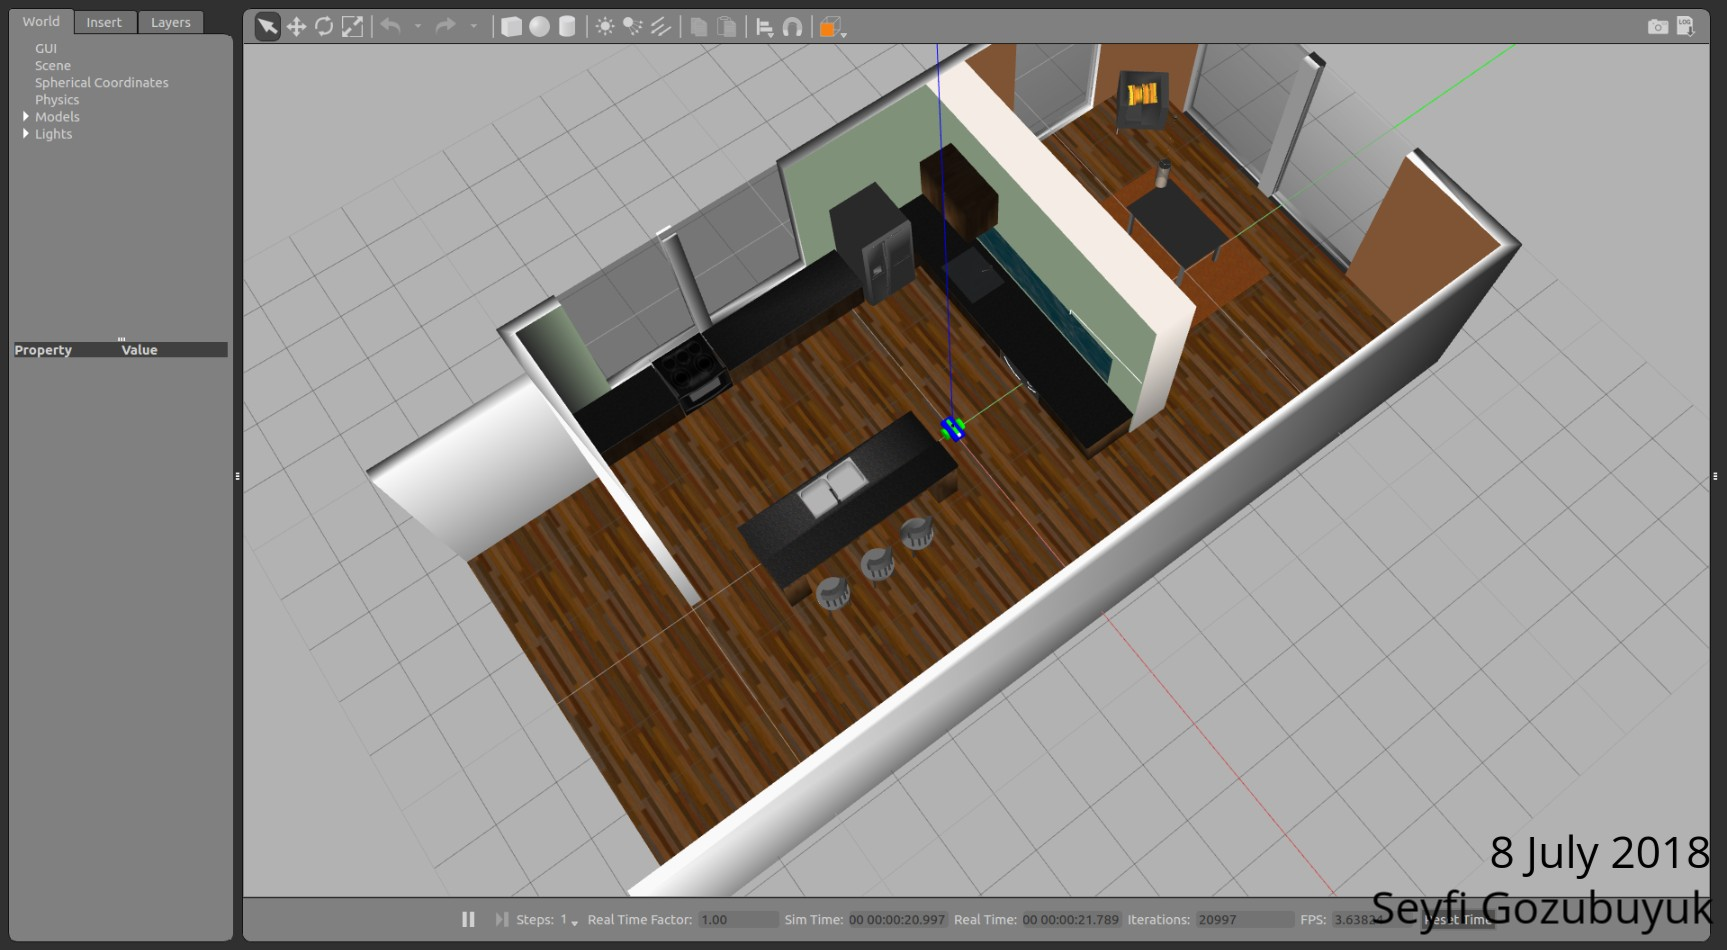
\includegraphics[width=\linewidth]{figures/gazebo_kitchen.png}
      \caption{Kitchen Dining in Gazebo}
      \label{fig:gazkit}
\end{figure}

\begin{figure}[thpb]
      \centering
      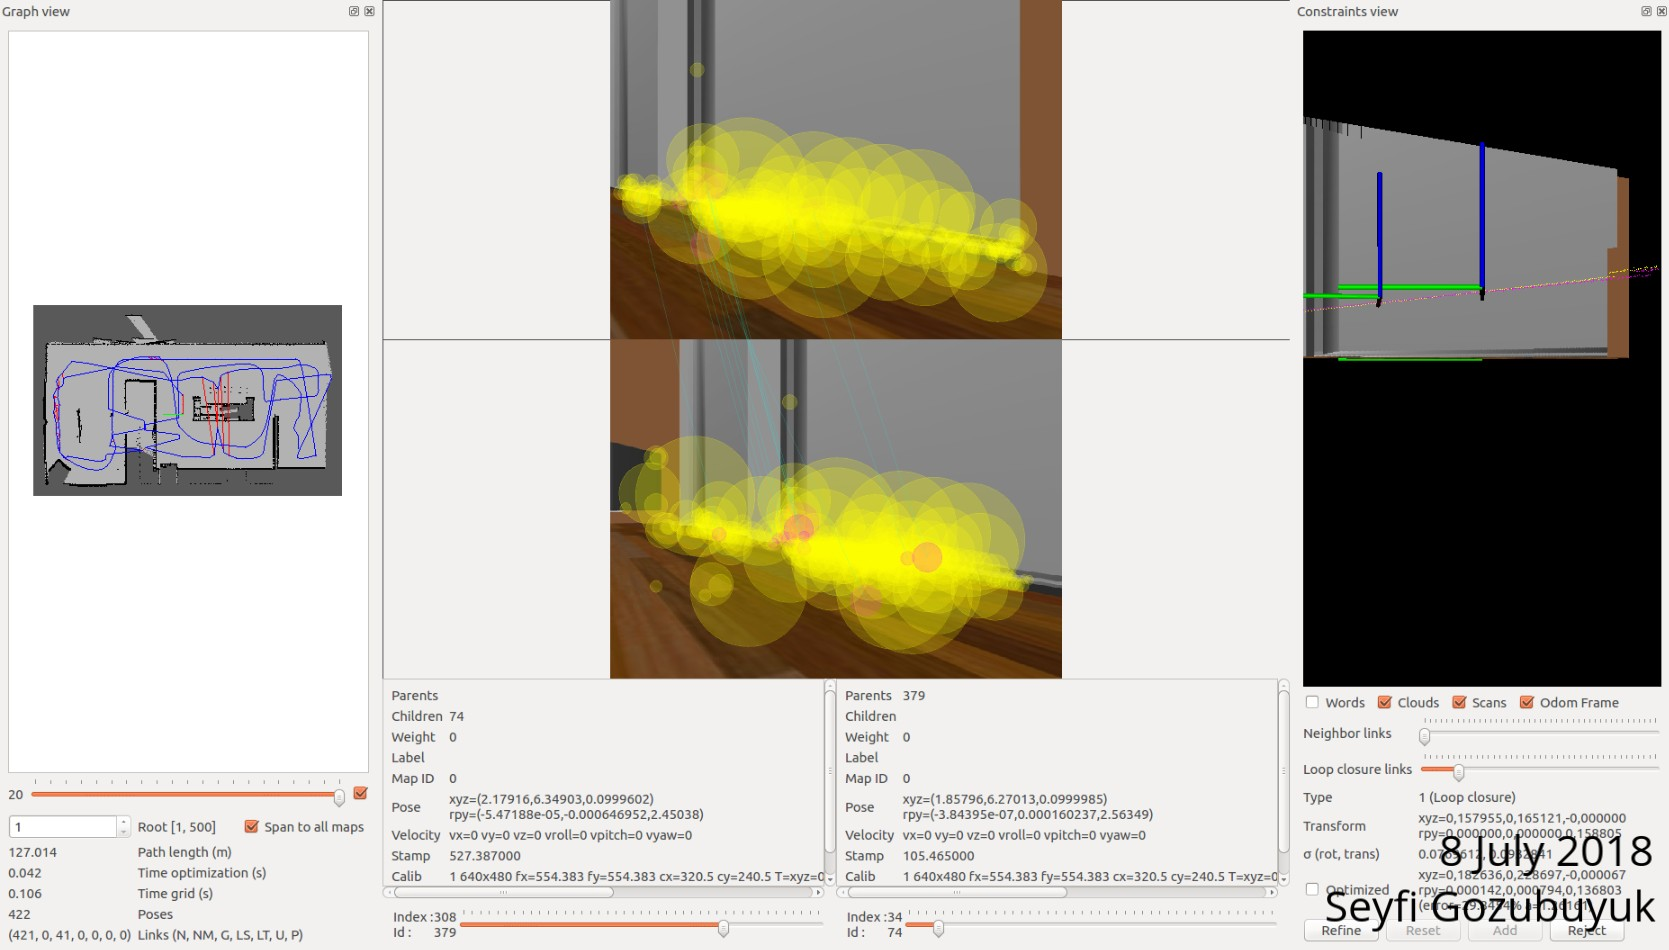
\includegraphics[width=\linewidth]{figures/rtabmap_kitchen.png}
      \caption{Kitchen Dining in RTABMap DB Viewer}
      \label{fig:rtbkit}
\end{figure}

\subsection{The X World}
The X World was built as the custom environment. To increase mapping accuracy, different types of objects were distributed to the map. Figure~\ref{fig:gazx} shows the custom world in Gazebo. The map from the mapping process is shown in Figure~\ref{fig:rvzx}. The screenshot from the RTAPMap database visualization is in the Figure~\ref{fig:rtbx}.

\begin{figure}[thpb]
      \centering
      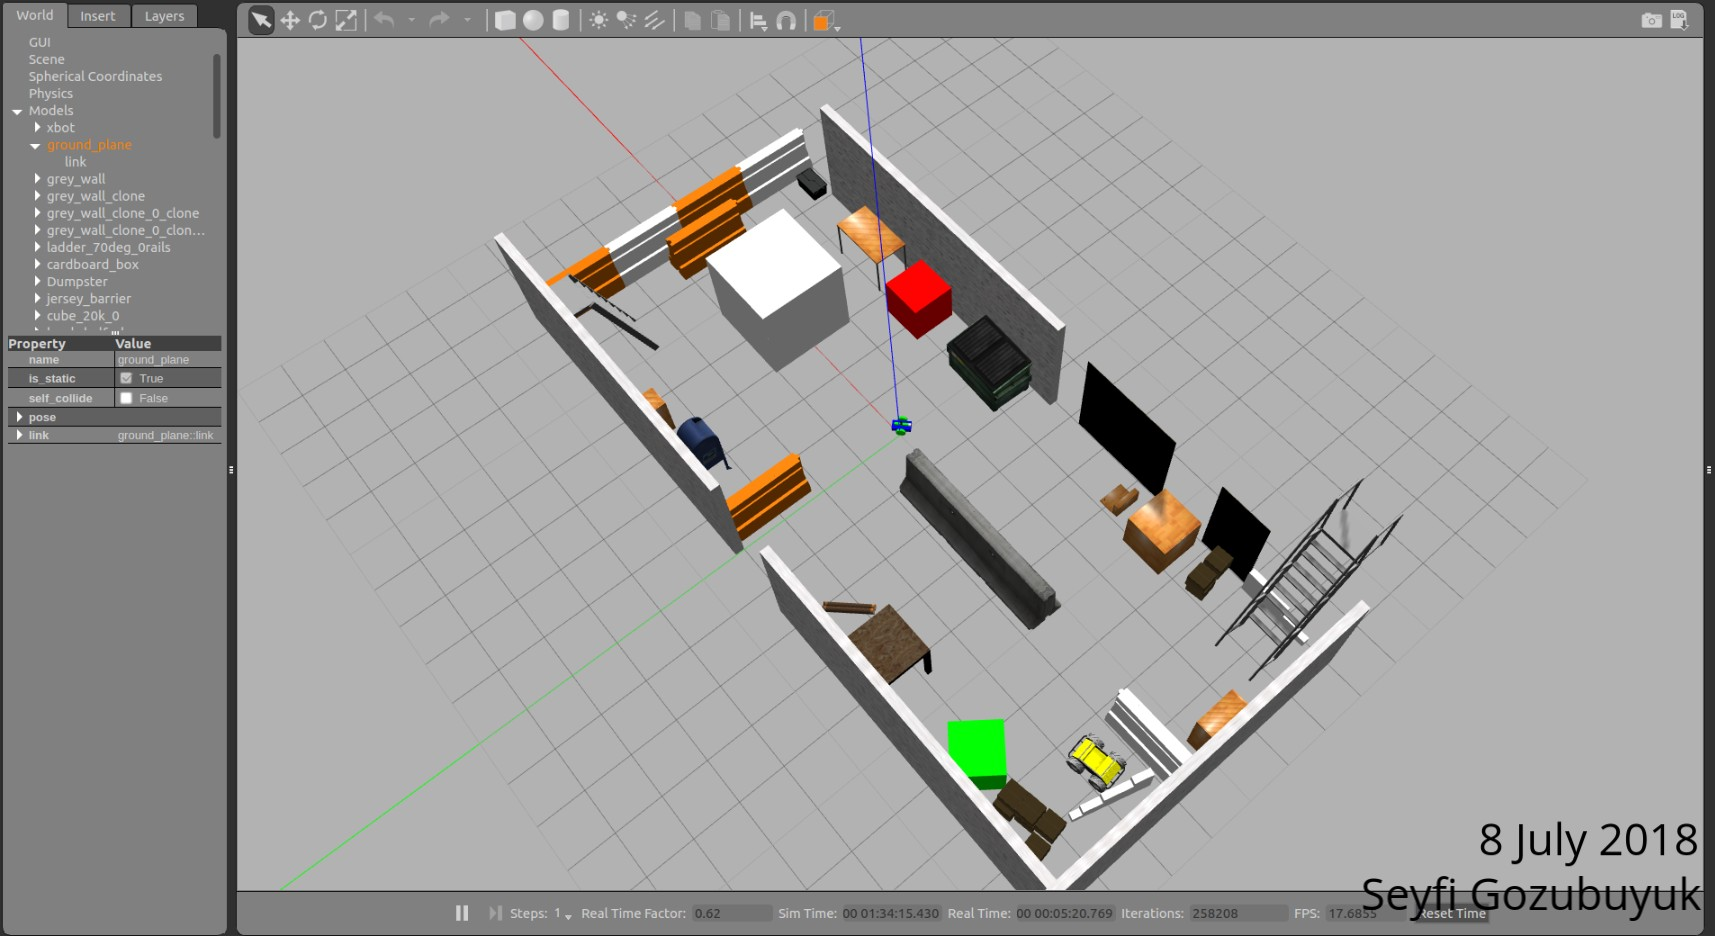
\includegraphics[width=\linewidth]{figures/gazebo_x.png}
      \caption{X World in Gazebo}
      \label{fig:gazx}
\end{figure}

\begin{figure}[thpb]
      \centering
      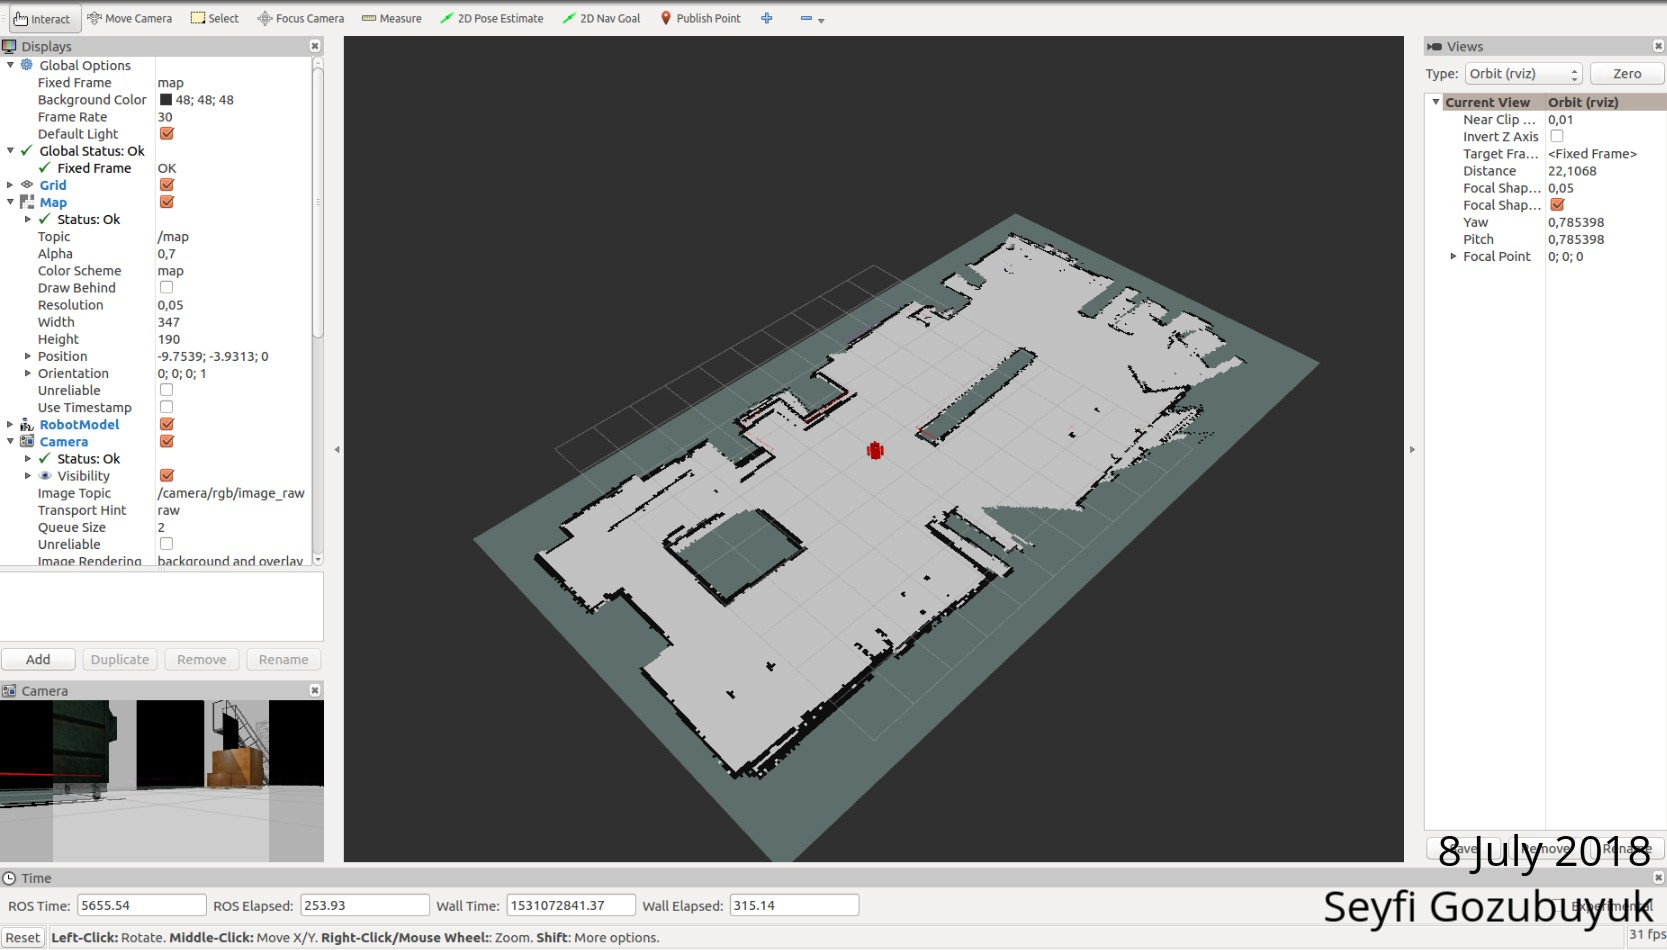
\includegraphics[width=\linewidth]{figures/rviz_x.png}
      \caption{X World in RViz}
      \label{fig:rvzx}
\end{figure}

\begin{figure}[thpb]
      \centering
      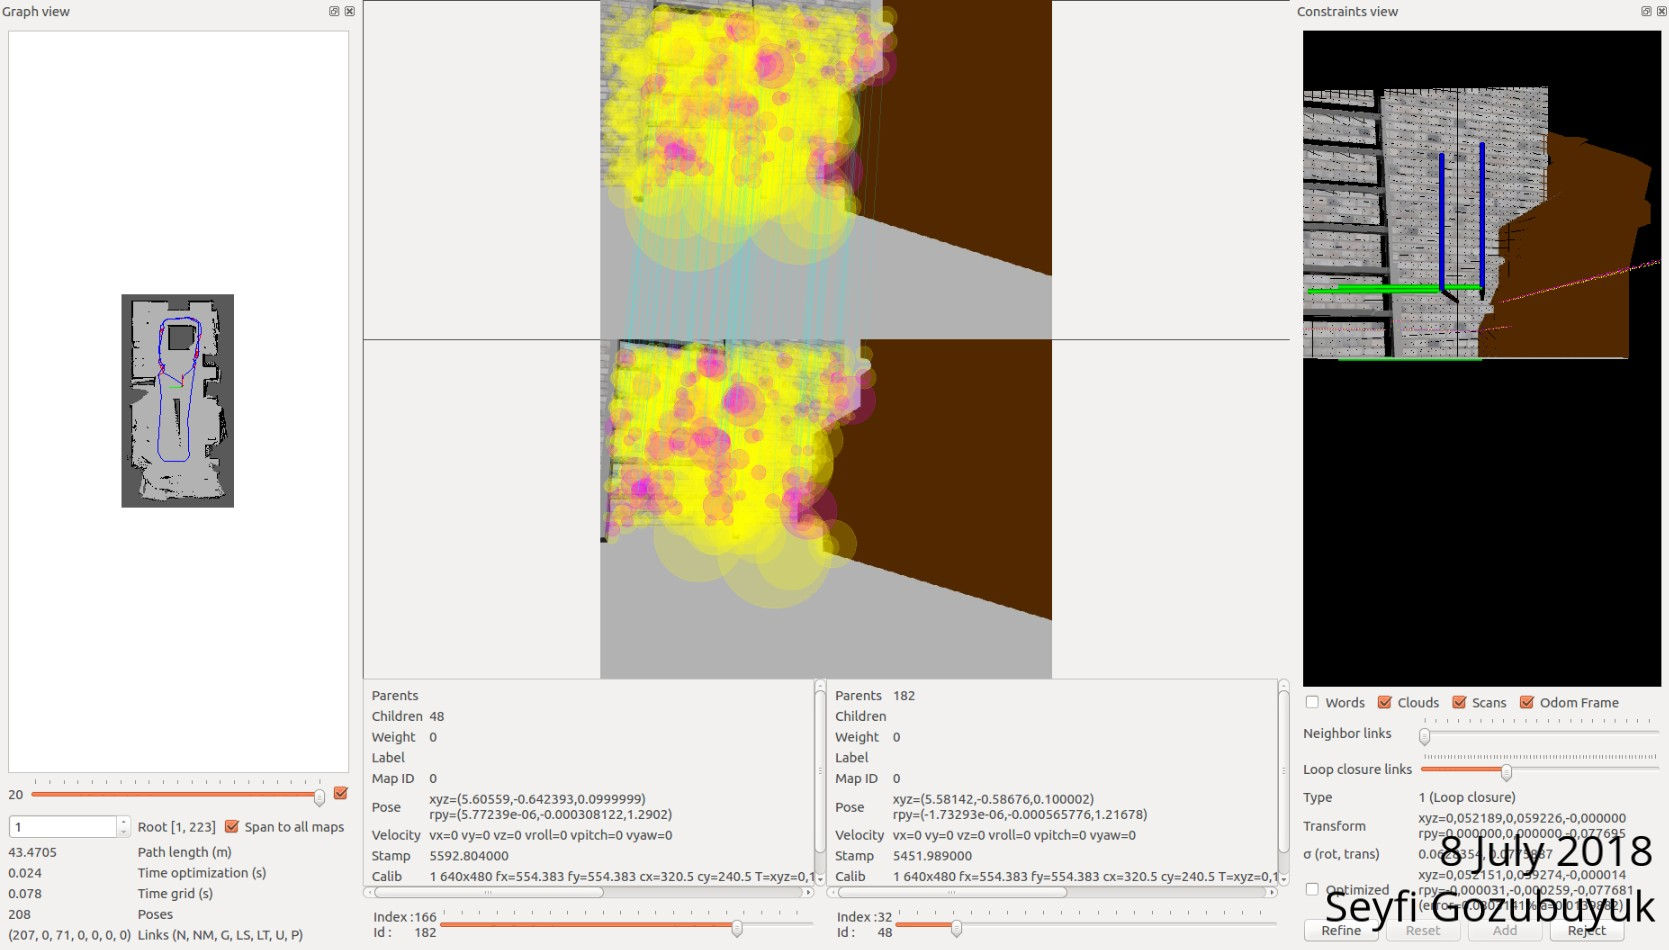
\includegraphics[width=\linewidth]{figures/rtabmap_x.png}
      \caption{X World in RTABMap DB Viewer}
      \label{fig:rtbx}
\end{figure}



\subsection{Achievements}
The algorithm was able to create maps for both of the environments, however, the maps were not perfect. There were little rotations and noises on the maps. Figure~\ref{fig:tff} shows the frame, and Figure~\ref{fig:rqt} shows the topics and the ROS graph.

\begin{figure}[thpb]
      \centering
      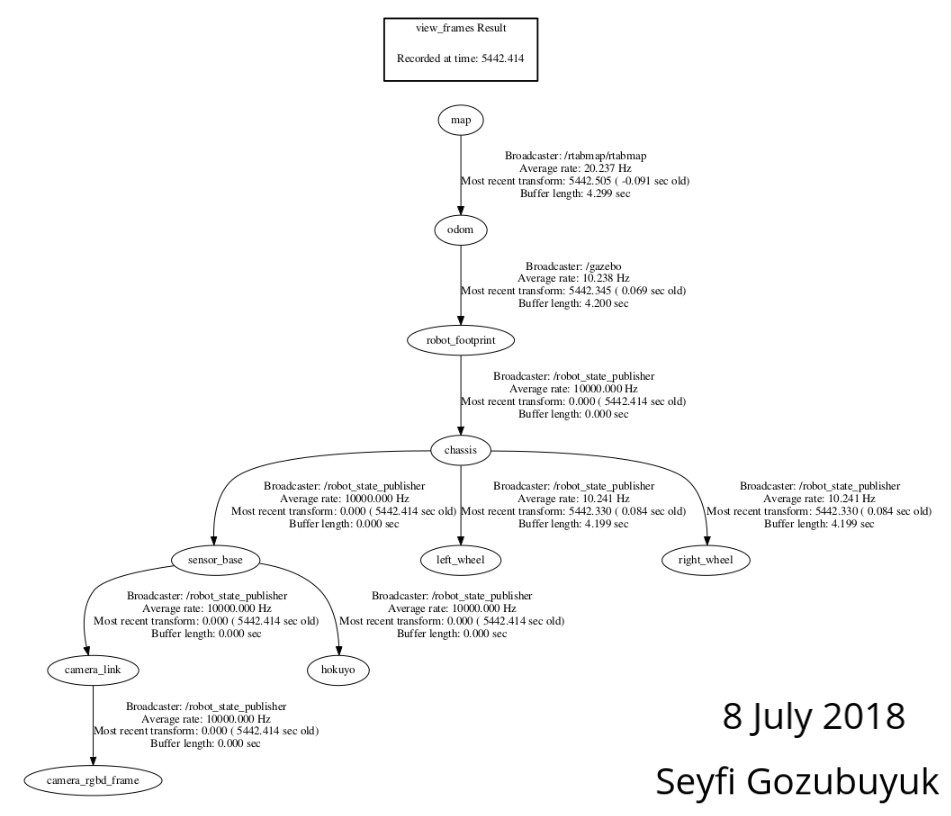
\includegraphics[width=\linewidth]{figures/tf_frames.png}
      \caption{TF Frames}
      \label{fig:tff}
\end{figure}

\begin{figure}[thpb]
      \centering
      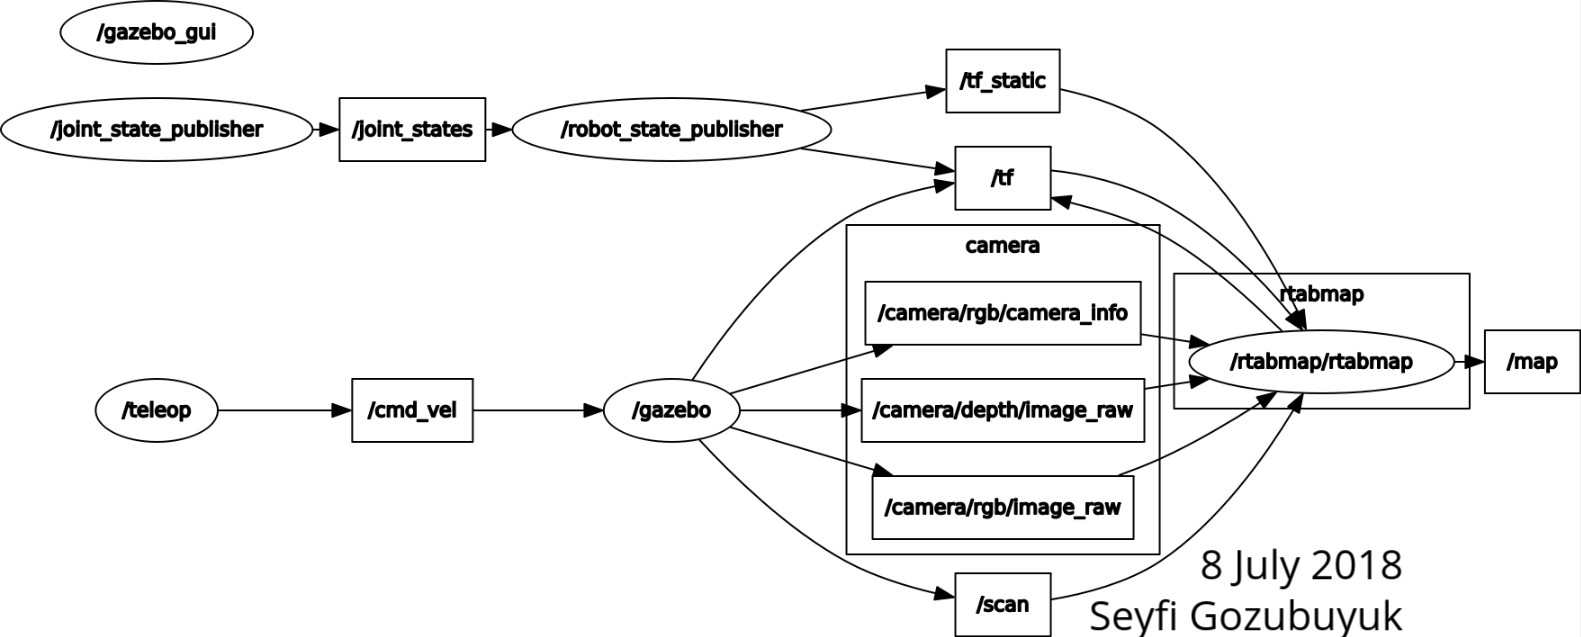
\includegraphics[width=\linewidth]{figures/rosgraph.png}
      \caption{ROS Graph and Topics}
      \label{fig:rqt}
\end{figure}

\section{Results}

\subsection{Mapping Results}
\subsubsection{The Kitchen Dining}
The map as an image file is shown in Figure~\ref{fig:mapkit}. The image file does not show an image as successful as the RTAPMap viewer. There exist rotations in the map.

\begin{figure}[thpb]
      \centering
      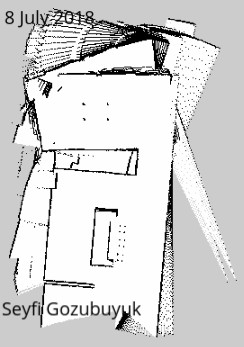
\includegraphics[width=\linewidth]{figures/map_kitchen.png}
      \caption{Kitchen Dining Map}
      \label{fig:mapkit}
\end{figure}

\subsubsection{xbot}
Figure~\ref{fig:mapx} shows the image file saved with map\textunderscore server map\textunderscore saver. Again, the saved map is not as successful as the image on the RTAPMap viewer. The map is skewed from the horizontal middle line.

\begin{figure}[thpb]
      \centering
      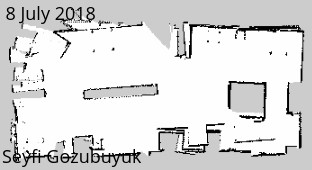
\includegraphics[width=\linewidth]{figures/map_x.png}
      \caption{X World Map}
      \label{fig:mapx}
\end{figure}

\subsection{Technical Comparison} % only facts
The first world is a more realistic world. It has objects to serve as landmarks which lead to a better mapping for the algorithm. There are several objects in the custom map, but still, it is harder to create the map of the x world.

\section{Discussion}
The algorithm was able to create a map for each environment. The robot navigated for almost two laps in both of the worlds. Both of the map images look warped. The parameters for the algorithm should be optimized, but due to time limitations, the tunning operation would be future work.

\section{Conclusion / Future work}
It is required to tune the parameters for mapping. Besides, a more complex environment should be created for further tests.
\\
Testing the algorithm on the Jetson TX2 and comparing the results with the current results is a waiting task for the future work. Upon receiving successful results, the algorithms in the project can be used on a real robot such a vacuum cleaner or an autonomous forklift.

\subsection{Hardware Deployment}
The project was deployed in the simulation environment. The machine has an I7 CPU, 8GB RAM, and 650M GPU. The configuration was able to run the project, but the algorithm and simulation become slower for complex worlds. With more powerful CPU and GPU, it will be possible to increase the complexity of the environment.\\
More powerful hardware will enable to test on different and larger custom worlds. Using a Jetson TX2 would increase the performance of this project.

\bibliography{bib}
\bibliographystyle{ieeetr}

\end{document}